% A birth-death tree (vermillion) and its contour (blue), revealed in stages.
% Coordinates follow the birth-exchanged tree of fig:cont-right-bdp in
% Paper01_AgeBDPVarEnv/sections/4_Contours.tex (x -> 21 - x), the default tree of the talk.
% Compile with: pdflatex "\def\stage{k}% A birth-death tree (vermillion) and its contour (blue), revealed in stages.
% Coordinates follow the birth-exchanged tree of fig:cont-right-bdp in
% Paper01_AgeBDPVarEnv/sections/4_Contours.tex (x -> 21 - x), the default tree of the talk.
% Compile with: pdflatex "\def\stage{k}% A birth-death tree (vermillion) and its contour (blue), revealed in stages.
% Coordinates follow the birth-exchanged tree of fig:cont-right-bdp in
% Paper01_AgeBDPVarEnv/sections/4_Contours.tex (x -> 21 - x), the default tree of the talk.
% Compile with: pdflatex "\def\stage{k}% A birth-death tree (vermillion) and its contour (blue), revealed in stages.
% Coordinates follow the birth-exchanged tree of fig:cont-right-bdp in
% Paper01_AgeBDPVarEnv/sections/4_Contours.tex (x -> 21 - x), the default tree of the talk.
% Compile with: pdflatex "\def\stage{k}\input{tree_contour.tex}"   (k = 1..5)
%   1 tree only            2 + contour            3 + extrema labelled
%   4 first ascent faded   5 everything after the first ascent faded
\documentclass[tikz,border=4pt]{standalone}
\usepackage{xcolor}
\usepackage{libertinus-otf}
\usepackage{unicode-math}
\setmathfont{STIX Two Math}
\definecolor{paper}{HTML}{FAFAFA}
\definecolor{treecol}{HTML}{D55E00}
\definecolor{contcol}{HTML}{0072B2}

% Opacity of the first ascent, of the rest of the contour, and of the extrema labels.
\ifcase\stage\or
  \def\ascop{0}\def\restop{0}\def\dotop{0}\or
  \def\ascop{1}\def\restop{1}\def\dotop{0}\or
  \def\ascop{1}\def\restop{1}\def\dotop{1}\or
  \def\ascop{0.15}\def\restop{1}\def\dotop{0}\or
  \def\ascop{1}\def\restop{0.15}\def\dotop{0}\fi

\begin{document}
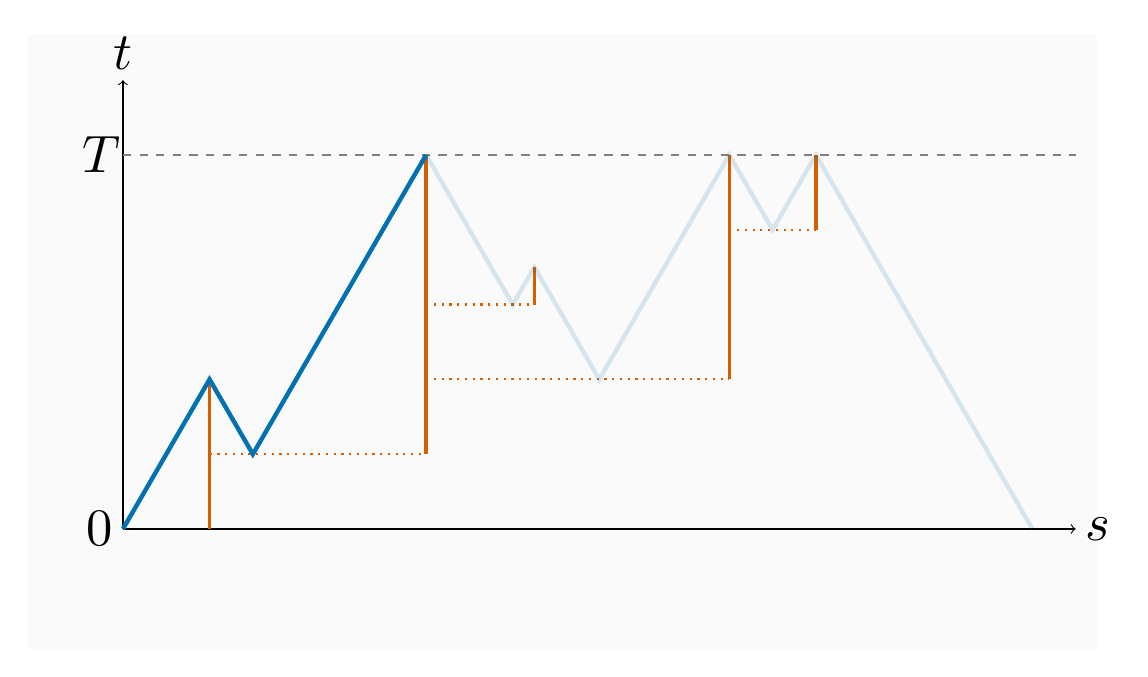
\begin{tikzpicture}[xscale=0.55, yscale=0.95, font=\fontsize{19pt}{23pt}\selectfont]
  % The same canvas for every stage, so stacked slides line up.
  \fill[paper] (-2.2,-1.6) rectangle (22.5,6.6);

  % Axes and the terminal level T
  \draw[->] (0,0) -- (22,0) node[right] {$s$};
  \draw[->] (0,0) -- (0,6) node[above] {$t$};
  \draw[dashed, gray] (0,5) -- (22,5);
  \node[left] at (0,5) {$T$};
  \node[left] at (0,0) {$0$};

  % The tree: vertical lifelines, dotted births
  \draw[very thick, treecol]
    (2,0) -- (2,2)
    (7,1) -- (7,5)
    (14,2) -- (14,5)
    (9.5,3) -- (9.5,3.5)
    (16,4) -- (16,5);
  \draw[thick, treecol, dotted]
    (2,1) -- (7,1)
    (7,2) -- (14,2)
    (7,3) -- (9.5,3)
    (14,4) -- (16,4);

  % The contour: first ascent to T, then the rest
  \draw[ultra thick, contcol, opacity=\ascop] (0,0) -- (2,2) -- (3,1) -- (7,5);
  \draw[ultra thick, contcol, opacity=\restop]
    (7,5) -- (9,3) -- (9.5,3.5) -- (11,2) -- (14,5) -- (15,4) -- (16,5) -- (21,0);

  % Extrema: X_1, X_3, ... peaks (deaths or T), X_2, X_4, ... valleys (births)
  \foreach \x/\y/\i/\pos in {2/2/1/above, 3/1/2/below, 7/5/3/above, 9/3/4/below,
      9.5/3.5/5/above, 11/2/6/below, 14/5/7/above, 15/4/8/below, 16/5/9/above,
      21/0/10/below} {
    \fill[contcol, opacity=\dotop] (\x,\y) circle (0.14);
    \node[\pos, contcol, opacity=\dotop, inner sep=2pt, font=\fontsize{15pt}{18pt}\selectfont] at (\x,\y) {$X_{\i}$};
  }
  \fill[contcol, opacity=\dotop] (0,0) circle (0.14);
  \node[below, contcol, opacity=\dotop, font=\fontsize{15pt}{18pt}\selectfont] at (0,0) {$X_0$};
\end{tikzpicture}
\end{document}
"   (k = 1..5)
%   1 tree only            2 + contour            3 + extrema labelled
%   4 first ascent faded   5 everything after the first ascent faded
\documentclass[tikz,border=4pt]{standalone}
\usepackage{xcolor}
\usepackage{libertinus-otf}
\usepackage{unicode-math}
\setmathfont{STIX Two Math}
\definecolor{paper}{HTML}{FAFAFA}
\definecolor{treecol}{HTML}{D55E00}
\definecolor{contcol}{HTML}{0072B2}

% Opacity of the first ascent, of the rest of the contour, and of the extrema labels.
\ifcase\stage\or
  \def\ascop{0}\def\restop{0}\def\dotop{0}\or
  \def\ascop{1}\def\restop{1}\def\dotop{0}\or
  \def\ascop{1}\def\restop{1}\def\dotop{1}\or
  \def\ascop{0.15}\def\restop{1}\def\dotop{0}\or
  \def\ascop{1}\def\restop{0.15}\def\dotop{0}\fi

\begin{document}
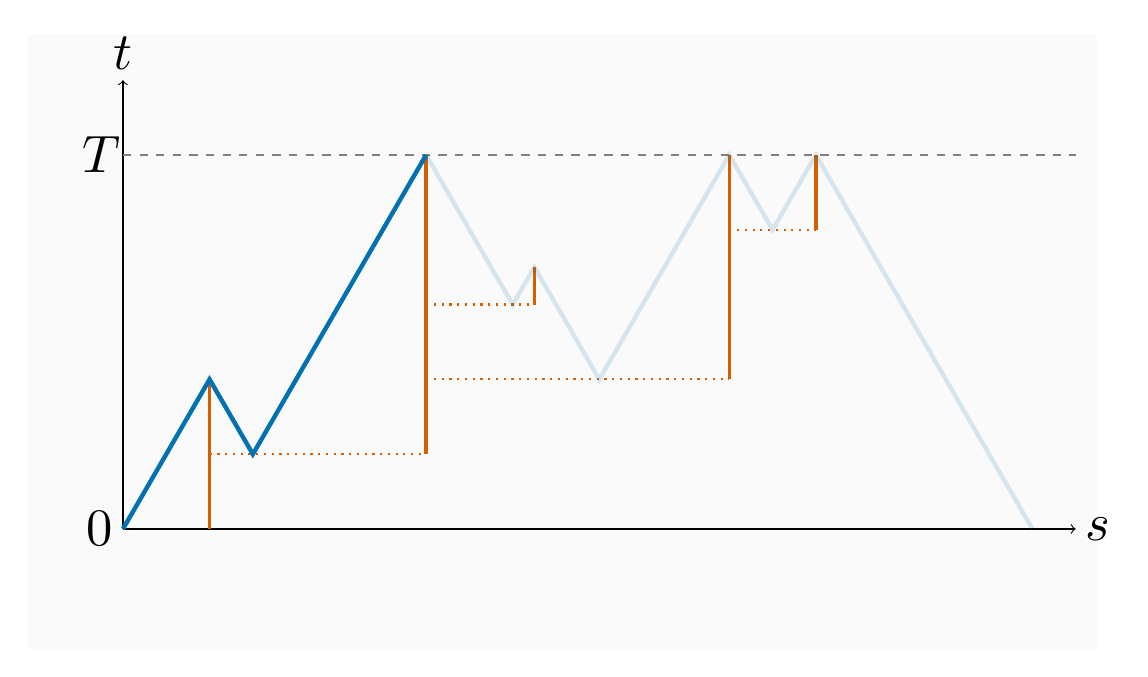
\begin{tikzpicture}[xscale=0.55, yscale=0.95, font=\fontsize{19pt}{23pt}\selectfont]
  % The same canvas for every stage, so stacked slides line up.
  \fill[paper] (-2.2,-1.6) rectangle (22.5,6.6);

  % Axes and the terminal level T
  \draw[->] (0,0) -- (22,0) node[right] {$s$};
  \draw[->] (0,0) -- (0,6) node[above] {$t$};
  \draw[dashed, gray] (0,5) -- (22,5);
  \node[left] at (0,5) {$T$};
  \node[left] at (0,0) {$0$};

  % The tree: vertical lifelines, dotted births
  \draw[very thick, treecol]
    (2,0) -- (2,2)
    (7,1) -- (7,5)
    (14,2) -- (14,5)
    (9.5,3) -- (9.5,3.5)
    (16,4) -- (16,5);
  \draw[thick, treecol, dotted]
    (2,1) -- (7,1)
    (7,2) -- (14,2)
    (7,3) -- (9.5,3)
    (14,4) -- (16,4);

  % The contour: first ascent to T, then the rest
  \draw[ultra thick, contcol, opacity=\ascop] (0,0) -- (2,2) -- (3,1) -- (7,5);
  \draw[ultra thick, contcol, opacity=\restop]
    (7,5) -- (9,3) -- (9.5,3.5) -- (11,2) -- (14,5) -- (15,4) -- (16,5) -- (21,0);

  % Extrema: X_1, X_3, ... peaks (deaths or T), X_2, X_4, ... valleys (births)
  \foreach \x/\y/\i/\pos in {2/2/1/above, 3/1/2/below, 7/5/3/above, 9/3/4/below,
      9.5/3.5/5/above, 11/2/6/below, 14/5/7/above, 15/4/8/below, 16/5/9/above,
      21/0/10/below} {
    \fill[contcol, opacity=\dotop] (\x,\y) circle (0.14);
    \node[\pos, contcol, opacity=\dotop, inner sep=2pt, font=\fontsize{15pt}{18pt}\selectfont] at (\x,\y) {$X_{\i}$};
  }
  \fill[contcol, opacity=\dotop] (0,0) circle (0.14);
  \node[below, contcol, opacity=\dotop, font=\fontsize{15pt}{18pt}\selectfont] at (0,0) {$X_0$};
\end{tikzpicture}
\end{document}
"   (k = 1..5)
%   1 tree only            2 + contour            3 + extrema labelled
%   4 first ascent faded   5 everything after the first ascent faded
\documentclass[tikz,border=4pt]{standalone}
\usepackage{xcolor}
\usepackage{libertinus-otf}
\usepackage{unicode-math}
\setmathfont{STIX Two Math}
\definecolor{paper}{HTML}{FAFAFA}
\definecolor{treecol}{HTML}{D55E00}
\definecolor{contcol}{HTML}{0072B2}

% Opacity of the first ascent, of the rest of the contour, and of the extrema labels.
\ifcase\stage\or
  \def\ascop{0}\def\restop{0}\def\dotop{0}\or
  \def\ascop{1}\def\restop{1}\def\dotop{0}\or
  \def\ascop{1}\def\restop{1}\def\dotop{1}\or
  \def\ascop{0.15}\def\restop{1}\def\dotop{0}\or
  \def\ascop{1}\def\restop{0.15}\def\dotop{0}\fi

\begin{document}
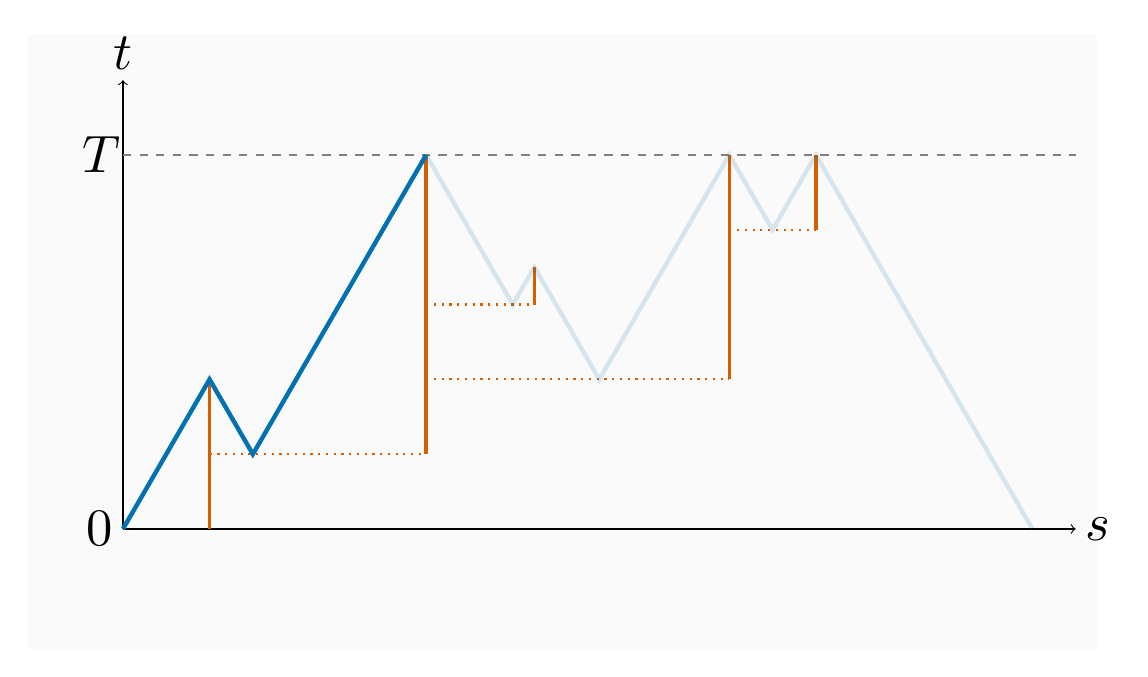
\begin{tikzpicture}[xscale=0.55, yscale=0.95, font=\fontsize{19pt}{23pt}\selectfont]
  % The same canvas for every stage, so stacked slides line up.
  \fill[paper] (-2.2,-1.6) rectangle (22.5,6.6);

  % Axes and the terminal level T
  \draw[->] (0,0) -- (22,0) node[right] {$s$};
  \draw[->] (0,0) -- (0,6) node[above] {$t$};
  \draw[dashed, gray] (0,5) -- (22,5);
  \node[left] at (0,5) {$T$};
  \node[left] at (0,0) {$0$};

  % The tree: vertical lifelines, dotted births
  \draw[very thick, treecol]
    (2,0) -- (2,2)
    (7,1) -- (7,5)
    (14,2) -- (14,5)
    (9.5,3) -- (9.5,3.5)
    (16,4) -- (16,5);
  \draw[thick, treecol, dotted]
    (2,1) -- (7,1)
    (7,2) -- (14,2)
    (7,3) -- (9.5,3)
    (14,4) -- (16,4);

  % The contour: first ascent to T, then the rest
  \draw[ultra thick, contcol, opacity=\ascop] (0,0) -- (2,2) -- (3,1) -- (7,5);
  \draw[ultra thick, contcol, opacity=\restop]
    (7,5) -- (9,3) -- (9.5,3.5) -- (11,2) -- (14,5) -- (15,4) -- (16,5) -- (21,0);

  % Extrema: X_1, X_3, ... peaks (deaths or T), X_2, X_4, ... valleys (births)
  \foreach \x/\y/\i/\pos in {2/2/1/above, 3/1/2/below, 7/5/3/above, 9/3/4/below,
      9.5/3.5/5/above, 11/2/6/below, 14/5/7/above, 15/4/8/below, 16/5/9/above,
      21/0/10/below} {
    \fill[contcol, opacity=\dotop] (\x,\y) circle (0.14);
    \node[\pos, contcol, opacity=\dotop, inner sep=2pt, font=\fontsize{15pt}{18pt}\selectfont] at (\x,\y) {$X_{\i}$};
  }
  \fill[contcol, opacity=\dotop] (0,0) circle (0.14);
  \node[below, contcol, opacity=\dotop, font=\fontsize{15pt}{18pt}\selectfont] at (0,0) {$X_0$};
\end{tikzpicture}
\end{document}
"   (k = 1..5)
%   1 tree only            2 + contour            3 + extrema labelled
%   4 first ascent faded   5 everything after the first ascent faded
\documentclass[tikz,border=4pt]{standalone}
\usepackage{xcolor}
\usepackage{libertinus-otf}
\usepackage{unicode-math}
\setmathfont{STIX Two Math}
\definecolor{paper}{HTML}{FAFAFA}
\definecolor{treecol}{HTML}{D55E00}
\definecolor{contcol}{HTML}{0072B2}

% Opacity of the first ascent, of the rest of the contour, and of the extrema labels.
\ifcase\stage\or
  \def\ascop{0}\def\restop{0}\def\dotop{0}\or
  \def\ascop{1}\def\restop{1}\def\dotop{0}\or
  \def\ascop{1}\def\restop{1}\def\dotop{1}\or
  \def\ascop{0.15}\def\restop{1}\def\dotop{0}\or
  \def\ascop{1}\def\restop{0.15}\def\dotop{0}\fi

\begin{document}
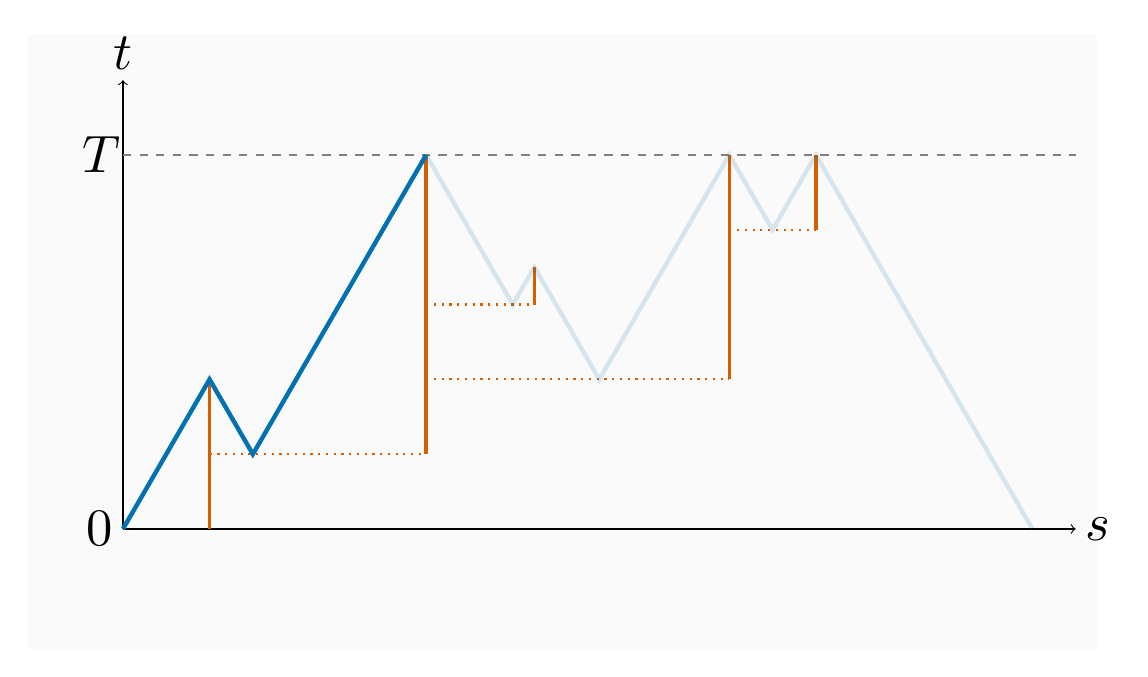
\begin{tikzpicture}[xscale=0.55, yscale=0.95, font=\fontsize{19pt}{23pt}\selectfont]
  % The same canvas for every stage, so stacked slides line up.
  \fill[paper] (-2.2,-1.6) rectangle (22.5,6.6);

  % Axes and the terminal level T
  \draw[->] (0,0) -- (22,0) node[right] {$s$};
  \draw[->] (0,0) -- (0,6) node[above] {$t$};
  \draw[dashed, gray] (0,5) -- (22,5);
  \node[left] at (0,5) {$T$};
  \node[left] at (0,0) {$0$};

  % The tree: vertical lifelines, dotted births
  \draw[very thick, treecol]
    (2,0) -- (2,2)
    (7,1) -- (7,5)
    (14,2) -- (14,5)
    (9.5,3) -- (9.5,3.5)
    (16,4) -- (16,5);
  \draw[thick, treecol, dotted]
    (2,1) -- (7,1)
    (7,2) -- (14,2)
    (7,3) -- (9.5,3)
    (14,4) -- (16,4);

  % The contour: first ascent to T, then the rest
  \draw[ultra thick, contcol, opacity=\ascop] (0,0) -- (2,2) -- (3,1) -- (7,5);
  \draw[ultra thick, contcol, opacity=\restop]
    (7,5) -- (9,3) -- (9.5,3.5) -- (11,2) -- (14,5) -- (15,4) -- (16,5) -- (21,0);

  % Extrema: X_1, X_3, ... peaks (deaths or T), X_2, X_4, ... valleys (births)
  \foreach \x/\y/\i/\pos in {2/2/1/above, 3/1/2/below, 7/5/3/above, 9/3/4/below,
      9.5/3.5/5/above, 11/2/6/below, 14/5/7/above, 15/4/8/below, 16/5/9/above,
      21/0/10/below} {
    \fill[contcol, opacity=\dotop] (\x,\y) circle (0.14);
    \node[\pos, contcol, opacity=\dotop, inner sep=2pt, font=\fontsize{15pt}{18pt}\selectfont] at (\x,\y) {$X_{\i}$};
  }
  \fill[contcol, opacity=\dotop] (0,0) circle (0.14);
  \node[below, contcol, opacity=\dotop, font=\fontsize{15pt}{18pt}\selectfont] at (0,0) {$X_0$};
\end{tikzpicture}
\end{document}
